\subsection{Questions, comparisons, and service accounting}
We evaluate how retained computation becomes continuously available
service, when an in-flight original call can be used, and how publication
and resource choices affect those benefits. The factorial study tests
joint computation/view retention; the native study repeats both switches
under the original recognizer--corrector task, with a no-speculation
anchor. Both record
actual Consumer applications and preserve every offered input obligation.

The core study uses Qwen3-ASR~1.7B~\cite{shi2026qwen3asr} on two 24-GB
RTX~3090s. Private and Authority workers use FP16 and FP32; batch delivery,
selection, validation, and persistence are shared. Twenty-four
metadata-selected LibriSpeech speakers~\cite{panayotov2015librispeech}
form three disjoint eight-speaker cohorts. The primary Qwen setting
offers 714.110~audio-s per arm, with 2-s feedback and arrivals staggered
by 0.25~s. Physical early exit is disabled.

Native execution uses two complete FP32 workers on the same two GPUs,
the original StreamCorrect ASR, correction, and update path
~\cite{vu2026streamcorrect}, and 500-ms inputs without VAD. The main
comparison crosses five policies with eight prespecified AISHELL-1
speakers~\cite{bu2017aishell}, one complete 8.138--9.000-s utterance each,
and two fresh repeats per policy; repeats stay within speaker pairs.

For offered interval $i$, duration $w_i$, ready time $r_i$, first actual
visible coverage $d_i$, and first original certified coverage $c_i$, we
report
\begin{equation}
 A_{2,8}=\sum_i w_i\,\mathbf{1}
 \{d_i-r_i\leq2\ \land\ c_i-r_i\leq8\}.
 \label{eq:credit}
\end{equation}
Every offered interval, including partial EOS tails and missing
observations, stays in the denominator. Whole-run passes require
offered-frontier display P99$\leq2$~s and certification P99$\leq8$~s.
Continued availability is measured separately from first delivery: a
withdrawal removes audio-seconds from an already-displayed view, and
the \emph{gap} integrates those removed audio-seconds over the wall
time they stay unavailable, so it is zero only when no displayed
coverage is erased.
Worker occupation sums elapsed worker-job intervals; both-board energy
runs from service origin through confirmed physical model drain.
Loading/warmup precedes normal service, while replacement and outstanding
work retain the original clocks. Reference generation is accounted
separately.

\subsection{Does retained computation remain available to the Consumer?}
We cross computation retention $R$ and supported-view retention $S$,
keeping selection authority and application safety checks common.
Table~\ref{tab:factorial_tradeoff} puts timely credit, withdrawal, and
gap in the same comparison. Relative to snapshot/recompute, computation-only
adds 1.41 percentage points of coverage but raises total withdrawals
from 12 to 17 (avoidable: 6 to 17). View-only reduces total withdrawals
to one and avoidable withdrawals to zero, while coverage falls by
3.60 points. Among these four arms, joint retention improves coverage
by 3.73 points and eliminates withdrawals
(Fig.~\ref{fig:main_evidence}).

\begin{table}[t]
\centering
\caption{Primary staggered factorial comparison: 714.110 offered
audio-s and 368 offered frontiers per arm. Withdrawals are classified
at the actual Consumer; the count in parentheses is the avoidable
subset. Gap is the time integral of removed, not yet restored
displayed audio.}
\label{tab:factorial_tradeoff}
\begingroup\small\setlength{\tabcolsep}{2.5pt}
\begin{tabular}{@{}lrrr@{}}
\toprule
Arm & $A_{2,8}$ (s) & Withdrawals & Gap (audio-s$\cdot$s)\\
\midrule
$R_0S_0$ Snapshot & 654.115 & 12 (6) & 15.458\\
$R_0S_1$ View only & 628.435 & 1 (0) & 0.258\\
$R_1S_0$ Compute only & 664.150 & 17 (17) & 30.258\\
$R_1S_1$ Joint & 680.760 & 0 (0) & 0.000\\
\bottomrule
\end{tabular}\endgroup
\end{table}

Withdrawals separate into two classes, and one class follows each
factor. A withdrawal is avoidable when the cleared view is compatible
with the projection that installs, and necessary when later feedback
contradicts that view. Necessary withdrawals are absent in both arms
that retain computation and present in both that do not (six and one);
avoidable withdrawals are absent in both arms that retain the view and
present in both that do not (six and seventeen). Only the joint arm is
empty in both, so coordination is not two gains added: it is the
intersection of two failure modes with different causes. The reason is
content rather than timing: an ahead view built by a complete call on a
frozen input can be overtaken in time but not contradicted in content,
whereas whether a compatible view survives application is a publication
decision.

Neither the count nor the credit fixes how long a reader loses text.
Under the snapshot baseline 12 withdrawals fall on the 368 offered
frontiers, 3.3 per 100, in all three cohorts; they remove 10.5~s of
already-displayed audio and keep it unavailable for
15.5 audio-s$\cdot$s. Computation retention raises the three
quantities to 17, 18.6~s, and 30.3. The gap sums both classes, which
is why view-only still shows 0.26: that residue is its single necessary
withdrawal, where later feedback contradicts a forecast view rather than
a compatible application. Joint retention has none of either class, and
the 2.176-s case of Figure~\ref{fig:continuity_case} is a sample of this
distribution rather than an outlier in it.

Credit is the service-level shadow of that structure. With
$I=Y_{11}-Y_{10}-Y_{01}+Y_{00}$ and $Y$ the credited audio, the three
initial primary staggered cohorts give $+18.530$, $+6.205$, and
$+17.555$~s; the mean sourcewise interaction is $+5.90$
percentage points, with a descriptive 95\% bootstrap interval of
$[1.13,10.28]$ over the 24 paired source effects. Credit aggregates one
run, so it also carries the timing of every offered interval, whereas a
withdrawal is classified at a single application.

% v18: per-cohort decomposition of the primary staggered factorial.
% Source: physical_retirement_20261028/H3_RESULTS_v2/aggregate/RUNS.json,
% phase=primary, adapter=qwen, rho=1, arrival=staggered, repeat=0.
\begin{table}[t]
\centering
\caption{Per-cohort decomposition of Table~\ref{tab:factorial_tradeoff}.
Each cell is dual-deadline credit (s) / avoidable withdrawals, over the
audio each cohort offers to all four arms; $I$ is the interaction
defined in the text.}
\label{tab:cohort_factorial}
\begingroup\footnotesize\setlength{\tabcolsep}{3.2pt}
\begin{tabular}{@{}lrrrrr@{}}
\toprule
Cohort (s) & $R_0S_0$ & $R_0S_1$ & $R_1S_0$ & $R_1S_1$ & $I$ (s)\\
\midrule
A (240.520) & 225.740/3 & 210.000/0 & 226.565/7 & 229.355/0 & $+18.530$\\
B (237.580) & 212.460/1 & 216.435/0 & 215.930/6 & 226.110/0 & $+6.205$\\
C (236.010) & 215.915/2 & 202.000/0 & 221.655/4 & 225.295/0 & $+17.555$\\
\midrule
All (714.110) & 654.115/6 & 628.435/0 & 664.150/17 & 680.760/0 & $+42.290$\\
\bottomrule
\end{tabular}\endgroup
\end{table}


No cohort drives the aggregate (Table~\ref{tab:cohort_factorial}).
Computation-only raises avoidable withdrawals in all three cohorts
(3$\to$7, 1$\to$6, 2$\to$4), and joint retention has the highest credit
of the four arms in all three (229.355, 226.110, 225.295~s).

\begin{figure*}[t]
\centering
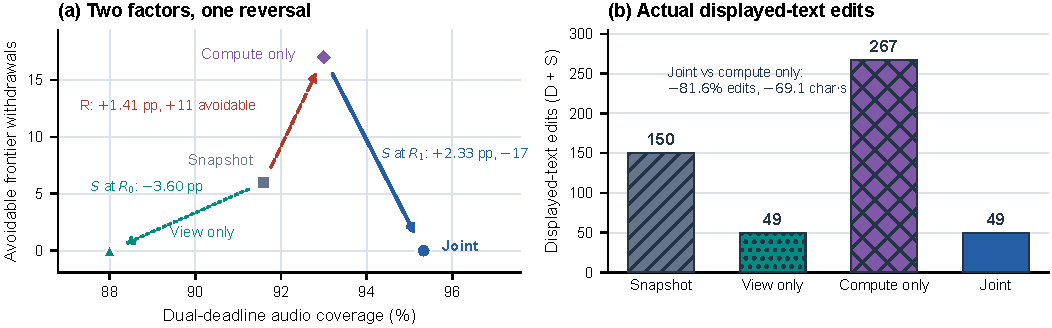
\includegraphics[width=\textwidth]{figures/core_interaction.pdf}
\caption{Joint retention preserves timely, supported progress (714.110
audio-s per arm, three eight-speaker cohorts, primary Qwen, 2-s
feedback, staggered; the four points are discrete policies, not a
measured continuum). (a) Arrows apply one factor: computation retention
alone (dashed) adds 1.41 points and 11 avoidable withdrawals, view
retention alone (dotted) removes six and gives up 3.60 points, both
(solid) gain 2.33 points and remove all 17. (b) Deletions/substitutions
under the primary minimum-distance alignment; final texts are identical
per source.}
\label{fig:main_evidence}
\end{figure*}

Complete dependency paths place each withdrawal at the application that
causes it: snapshot/recompute's 12 split six and six; computation-only's
17 are all avoidable, or 4.6 per 100 offered frontiers; and joint
retention preserves all 18
compatible-ahead opportunities it meets.

A separate 16-session workload makes that distinction visible when
first-delivery credit ranks the policies oppositely: in its third repeat
computation-only credits 201.960~s against 194.735~s, because two 2-s
intervals are withdrawn after credit is assigned. At eight staggered
sessions all arms pass whole-run $D_2/C_8$, yet computation-only still
loses timely supported coverage in 1/2/1 windows and joint retention in
none.

Text revision is another distinct outcome. On actual Consumer strings,
a minimum-distance Unicode alignment gives 267 deletions/substitutions
for computation-only and 49 for joint retention, with modified-identity
lifetimes of 203.297 versus 134.207~character-s, and an alternative
optimal alignment preserves the direction. Joint retention also retires
569 LCP-suffix characters. Final actual text hashes agree per source
across arms, and all five executed arms retain identical complete
selected frontier, result, state, and text histories within each
source/block.

\subsection{What does each switch contribute on the native path?}

\begin{figure*}[t]
\centering
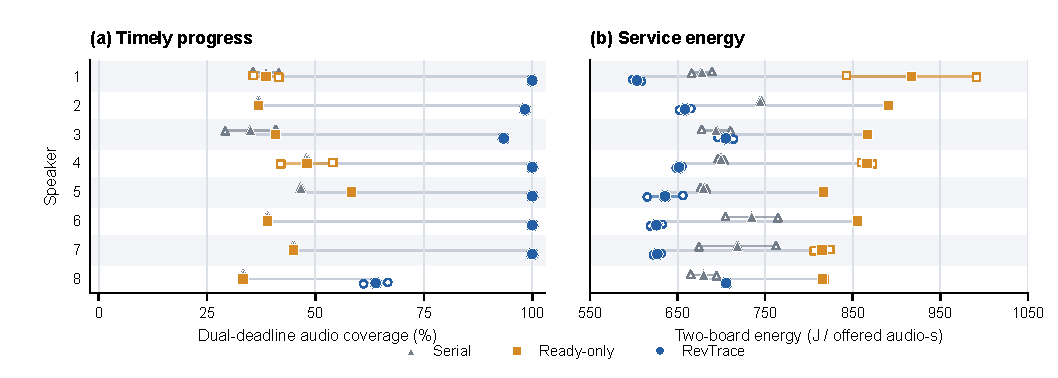
\includegraphics[width=\textwidth]{figures/native_comparison.pdf}
\caption{Timely progress and service energy on the eight-speaker native
workload. The three policies all retain whole supported views; they differ
in whether calls are serial, reusable only after completion, or retained
in flight. These are the same trials as Table~\ref{tab:native_confirmation_v16}:
two fresh-process repeats per speaker and policy from the 80-trial
factorial campaign. Filled markers pool the two repeats; open markers and
short ranges show the individual observations. Speakers use the same
order in both panels. (a) Audio meeting both the 2-s display and 8-s
certification deadlines. (b) Both-board energy from service origin to
confirmed physical model drain, divided by offered audio duration.}
\label{fig:native_comparison}
\end{figure*}
The native comparison isolates a call whose input becomes confirmed while
it is still running. \emph{Fullcall} ($R_1S_1$) keeps that original
complete call; \emph{Ready-only} ($R_0S_1$) can reuse a received,
validated result at the confirmation boundary, but fences an unresolved
call and reissues the work. Both share complete-input checks, original
C/U selection, whole-view support, two workers, ahead limits, and a
canonical-first round-robin dispatcher. The campaign runs each switch in
both positions, plus a policy that issues nothing before confirmation,
on the same eight speakers and 282 offered frontiers.

In-flight retention earns \NativeFullCreditPct\% of the 137.864~offered
audio-s per policy, against \NativeReadyCreditPct\% for completed-result
reuse and \NativeConsCreditPct\% for serial execution: 51.83 points over
reuse and 54.01 over no speculation. All eight sources move the same way
at both view settings, and the paired diagnostic is $2/256=0.0078$ for
each, the smallest value attainable with eight sources.

Fencing is not what produces the gap, and reuse is exercised. At this
500-ms cadence a fenced call's reissued work can display only after
confirmation plus a full inference, so a completed result is rarely
ready in time; one was, on S0907, and was reused. Its 3.000-audio-s
margin over no speculation therefore prices readiness rather than
fencing, at 65\% more worker time.

The two switches act on different quantities. At fixed view retention
the call is worth 71.460~s; at fixed call retention the view is worth
$-1.000$~s; the interaction is $-1.500$~s, so this runtime does not
establish a positive first-credit synergy. What it establishes is the
classification. Replacing the view clears all 10 compatible ahead views
the retaining call meets, on three of the eight sources, and all 13 when
the call is fenced; keeping the view clears none in either position.
Joint retention still withdraws twice, on S0902 in both repeats, where a
new canonical boundary refutes the old prediction: it withholds
incompatible views rather than all withdrawals.

Retained credit hides loss here as well. In-flight retention with the
replacing view earns 130.960~s, 1.000~s more than joint retention, while
removing 5.000~s of supported displayed audio in ten windows of
32--134~ms (median 63) and leaving 0.379~audio-s$\times$wall-s of
avoidable absence; joint retention's only removals are the two refuted
views, and its avoidable absence is zero. All 39 loss windows in the
campaign return within the same root, none censored or truncated. Which
arm leads on first credit is thus workload-dependent, as in the core
study; the class each switch removes is not. Avoidable withdrawal is not
rarer here, only shorter: it occurs at 3.5 per 100 offered frontiers
against 4.6 in the core study, and its length is set by when the next
compatible application arrives.

Worker occupation is \NativeFullWorkerSeconds~s against
\NativeReadyWorkerSeconds~s, and both-board energy is 89.848 against
117.826~kJ: reductions of 31.8\% and 23.7\% against reuse. Against
serial execution the trade partially reverses, because retention spends
12.6\% more worker time (222.523 versus 197.573~s) to serve the same
stream earlier while using 7.4\% less two-board energy (89.848 versus
96.985~kJ). The two comparisons answer different questions and are not
one dominance claim. Relative to Ready-only, every source improves on
credit and energy after pooling its two repeats
(Fig.~\ref{fig:native_comparison}).

\begin{table}[t]
\centering
\caption{Native retention policies: eight speakers, two fresh repeats,
137.864~audio-s and 282 offered frontiers per policy. R0 uses received
complete results only; R1 also keeps a call whose input is confirmed
while it runs. S0 replaces the whole view at a canonical application;
S1 keeps it when the support check passes. Conservative issues no work
ahead of confirmation. Work is occupied-worker wall time; energy covers
both boards to confirmed physical model drain.}
\label{tab:native_confirmation_v16}
\scriptsize\setlength{\tabcolsep}{2.4pt}
\begin{tabular}{@{}lrrrrrr@{}}
\toprule
Policy & $A_{2,8}$ (s) & Cov. & Pass & Av./Nec. & Work (s) & kJ\\
\midrule
Conservative & 55.500 & 40.26\% & 0/16 & 0/0 & 197.573 & 96.985\\
$R_0S_0$ & 58.000 & 42.07\% & 0/16 & 13/6 & 326.546 & 118.632\\
$R_0S_1$ & 58.500 & 42.43\% & 0/16 & 0/6 & 326.232 & 117.826\\
$R_1S_0$ & 130.960 & 94.99\% & 10/16 & 10/2 & 222.646 & 92.814\\
$R_1S_1$ & 129.960 & 94.27\% & 10/16 & 0/2 & 222.523 & 89.848\\
\bottomrule
\end{tabular}
\end{table}


Credit and whole-run passing retain different resolution. S0901 misses
$D_2$ only at EOS; S0902 misses twice at EOS and twice mid-utterance;
S0915 supplies 11 of the 13 non-EOS misses, which is why joint retention
passes 10/16 runs against 0/16 for Ready-only. No arm misses $C_8$ in
these 80 runs, so every miss in Table~\ref{tab:native_confirmation_v16}
is a display miss; the shorter bank never makes the deadline bind.



An earlier two-policy campaign on the same speakers reproduced aggregate
credit within 0.500~audio-s (129.460 against 129.960) and the same 10/16
passes, with 20 against 19 $D_2$ misses.

\subsection{Where the certification deadline binds}

Longer inputs expose it. On a second natural corpus---the lexicon first
four of 29 qualifying MAGICDATA Mandarin speakers~\cite{magicdata68},
one complete 14.396--15.232~s utterance each, frozen before any
transcript is read, three policies twice per speaker over 119.844~audio-s
and 244 frontiers---serial execution misses $C_8$ 27 times at up to
11.508~s, and both retaining arms miss it zero times, at 6.962 and
6.473~s. All 27 are $D_2$ misses as well, so the gain is a deadline met
rather than new $A_{2,8}$ intervals.

The same corpus separates the two retentions where credit cannot: both
earn 65.29275~audio-s against 38.000 for serial execution, identical to
the last digit, yet computation-only clears five compatible ahead views
that joint retention keeps and removes 2.500~audio-s of supported
display. AISHELL separated the arms by 1~s of credit; here only
availability tells them apart.

Serving earlier here costs 35.3\% more worker time and 13.3\% more
energy than serial execution, and all 24 runs reproduce the original
reference state, correction, and returned IDs.

\subsection{Which evidence permits retained work to be used?}
Among 92 model-active input confirmations in an earlier four-source
bank, 20 calls' tentative successor states differ from their final
original C/U results: inputs become valid while predictions are revised,
and retaining the computation leaves selection to the original program.

The six-policy, two-speaker pilot measures the corresponding execution
opportunity. Its 24 cells bind 1,200 actual Consumer rows to original
facts and received ASR/full-result paths. Fullcall has 56 model-active
handovers, each spanning the actual parent-receipt-to-install interval
and later selected for use. Ready-only has zero complete-result hits in
this pilot and 56 same-input reissues. Nine times, a complete result
finished only after its frontier had been fenced and was refused;
retaining the call would have used it.
Over 33.11625~offered audio-s per policy, Fullcall earns 32.340125~s
versus 12.5~s for Ready-only, with 51.765 versus 82.145~worker-s.

The \emph{dependency-versioned} policy realizes the same 56 handovers
and the same credit as Fullcall. Shadow predicates evaluated on the
five speculative policies' recorded schedules agree at all 290 sampled
job/install boundaries: 278 current-input matches and 12 refutations.
A state-bound version representation can therefore implement the same
input witness. The birth-root-fenced auxiliary
records no promotion and earns 12.000~s, equal to Conservative in this
pilot, because it revokes a call when its birth root changes even if the
complete input is later confirmed.

\emph{Unconditional in-flight retention} (UIR) refuses the same two
known-wrong complete returns but suppresses early skip hints; Fullcall
exits before learned correction there and earns 1.5~s more, both on
S0901. The trace thus separates refusal from resource outcome.

\subsection{Can agreement-based publication compose with retention?}
We adapt LocalAgreement-2's consecutive-new-input prefix
decision~\cite{machacek2023whisperstreaming} above the actual recorded
pilot candidates. Original ASR already uses AlignAtt~\cite{papi2023alignatt};
C/U, retained computation, and selected $G$ stay fixed. The adapter
compares Unicode code points and maps a stable prefix to an actually
delivered whole view with a supported complete path. Its audio frontier
comes from that view. Same-frontier ASR/full-C publications supply one
new-input update, and EOS release waits for actual final C/U delivery.

Here canonical-only gates first publication of provisional results;
the core $S$ factor instead governs retention at canonical application.
On Fullcall's four fixed schedules, actual-SUP credit is 32.340125~s,
canonical-only 30.840125~s, and LA2-CP 31.340125~s, over 33.11625~s.
LA2-CP removes all four modified characters for 1~audio-s of credit,
and its within-D2 coverage integral falls from 32.740 to
24.403~audio-s$\times$wall-s under the same right-censored allowance; a
0.5-s fixed-lag control yields 26.840~s, nine modified characters, and
three frontier retreats. The publication choice therefore trades
delivery timing against revision and coverage duration. The observer evaluates four rules on 24 recorded schedules and passes 28
unit tests.

\subsection{Which workloads provide useful retention opportunities?}
At two synchronous native sessions, Fullcall earns 11.5~s versus
Conservative's 10.5~s over 33.11625~s; at four, it earns 9~s versus
10~s over 66.91~s. All eight runs fail whole-run D2. Conservative can
occupy both GPUs with independent canonical chains, and the shared
canonical-first dispatcher issues no conditional work in the four-session
Fullcall cells. Available resources and competing canonical demand
determine whether that execution supplies in-flight work to retain.

Credit reverses under fresh timing: a staggered cohort-A run gives joint
retention 226.320~s against 230.565~s, and pooled synchronous arrivals
$-0.790$~s with $I=+2.565$~s, while it still preserves five and three
compatible-ahead opportunities. Credit tracks timing; which class a
factor removes does not.

\subsection{Do the checks preserve the intended authority?}
The native reference and Consumer checks bind complete inputs, original
C/U, and received whole-view paths. The CPU protocol suite passes
225 unit tests. A bounded hand-written model passes 35 named checks, including
its 27 original controls, over dispatch, ASR, original-C/U, durable-install,
and Consumer actions. Actual process-failure trials separately retain
two matching acquired complete results through producer exit and refuse
two mismatches against their actual parents. Together these checks
exercise the declared trust and ownership boundaries; the original
program, complete-state adapter, and synchronized storage remain their
trusted interfaces.

\subsection{What does the complete synchronous path cost?}
Eight instrumented native trials measure the complete fact and
Consumer paths. The observed mean commit takes 20.35--27.25~ms, or
4.1--5.5\% of the 500-ms input interval; 15.78--22.18~ms lies inside
its synchronous filesystem call, and a whole-view Consumer application
takes 18.58--23.91~ms. These operations bind the complete original
result and parent, persist the selected transition, and apply it to the
actual view that the end-to-end comparisons above measure.
